

\chapter{Discussion}
\label{Discussion}
\minitoc

\vspace*{0.3cm}

The treatment planning results presented in the previous chapters are the first feasibility study to investigate the use of carbon ions 
for a non-invasive treatment of atrial fibrillation (AF). Currently existing treatment procedures for this cardiac arrhythmia have major 
drawbacks and due to the prevalence of this condition a new treatment modality would be beneficial \cite{Cap05, Cap10}. It could 
be shown that scanned ion beams have the potential to become an accurate, fast and non-invasive treatment approach for AF.\newline 
\newline
Cardiac target volumes like the pulmonary veins (PVs) or the atrioventricular (AV) node move due to respiration of the patient as well as due 
to heartbeat. When treating moving targets with a scanned carbon ion beam interference effects between the particle delivery and the 
interfractional target motion are observed, leading to over and under dosages in the target volume and hence endangering the treatment outcome. 
Motion mitigation techniques are thus needed, which were studied independently for the respiratory and heartbeat motion influence. 
Cardiac target volumes are surrounded by critical structures and organs at risk (OAR) like esophagus, trachea and aorta. 
A detailed analysis of the OAR dose depostion was carried out, which will be discussed in section \ref{diss:Dose:OAR}. In section 
\ref{Dose:OAR:photons} special emphasis will be given to the reduced OAR dose deposition with scanned carbon ions compared to a non-invasive 
treatment with photons. The target volume displacement will be discussed in section \ref{diss:motion}. Afterwards the findings of treatment 
planning studies with motion mitigation techniques will be discussed in section \ref{diss:mmt}.

\newpage

\section{Dose deposition}

In the here presented feasibility study of a non-invasive treatment of AF with carbon ions, a physical dose of 25Gy was 
applied in all treatment plans. This dose was chosen according to the publication by Sharma et al. \cite{Sha10}  
in which it was stated as the minimal needed dose in order to see an electrophysiological effect induced by photon irradiation. 
Older studies with photon irradiations in animal models support the finding by Sharma et al. in which doses higher than 20Gy seem 
to be sufficient in order to induce fibrotic tissue \cite{Faj70, Faj73}. A short overview will be given in section \ref{Dose:Target}.\newline
\newline
A close analysis of the dose deposition to the OARs was carried out in the here presented work. Human data was studied for PVs ablation 
(chapters \ref{chapter:mdacc} and \ref{chapter:human}). In preparation for animal studies, which will be carried out at GSI in 2014, the 
irradiation of the AV node in pigs was analyzed (chapter \ref{chapter:porcine}). The findings will be discussed in section \ref{diss:Dose:OAR} 
and a comparison with photon irradiation will be given in \ref{Dose:OAR:photons}. For critical structures like the aorta, esophagus, trachea 
and the heart itself dose-volume limits from SBRT were used \cite{RTOG0631, RTOG0915}. As the heart is not only an OAR in this studied 
treatment, but the target site itself, the dose-volume limits for this organ were often exceeded. Closer analysis of the irradiated cardiac 
substructures was hence performed.  



\subsection{Dose to target area}
\label{Dose:Target}

Sharma et al. stated that a dose of at least 25Gy is needed in order to induce a change in the conduction system of the heart with photon 
beams \cite{Sha10}. Nevertheless also higher doses have been applied in the animal model study, reaching up to 80Gy. 
Part of the planned animal experiments at GSI will be a dose escalation study, in which the needed carbon ion dose for the 
generation of the desired fibrosis in the target area will be examined more closely. 
It is already known from former studies on the effect of radiation on the heart which dose depositions as single fraction doses are sufficient 
in order to induce fibrotic tissue \cite{Faj70, Faj73, Phil64, Bis65, Ste68, Efs56}.\newline
\newline
Fajardo et al. \cite{Faj70, Faj73} investigated the evolution of radiation induced myocardial damage after a single dose 
of 20Gy in rabbits as well as a fractionated treatment, both with 6MV photons. They stated that their findings were independent of the 
time course of the irradiation, hence if the dose was applied as a single fraction or in different fractions. They found that there are three 
distinct stages in the evolution of radiation induced cardiac damage and divided it into an acute phase (an inflammtion within the first 
48hours), a latent stage (which can last up to seventy days) and the late stage where fibrotic lesions occur. Their explanation for the formation of fibrotic 
tissue is a failure of microcirculation, resulting from a failure of the complete reconstruction of capillaries in the endothelial cells after 
irradiation. They state that the occuring ischemia leads to myocardium fibrosis, which becomes maximal beyond 120 days.
Other studies by Phillips et al. \cite{Phil64} and Bishop et al. \cite{Bis65} irradiated hearts of dogs and rodents with single photon doses 
of 60Gy to 96Gy. Both authors stated that they found severe functional abnormalities as well as myocardial 
fibrosis or even necrosis \cite{Ste68}. Efskind et al. \cite{Efs56} found fatal myocardial damage after 80Gy photon irradiation to the heart 
of rabbits.\newline
\newline
It can thus be assumed that the required dose for the desired generation of fibrotic tissue in the cardiac target volumes 
will require at least 20Gy, while high single fraction doses of up to 60Gy might induce necrosis, which needs to be avoided.
Preliminary studies using the LEM for the calculation of biological doses in single fraction deliveries with the stated 25Gy resulted to have 
a RBE of 1.1. This needs to be verified. Nevertheless studies exist, where the RBE was found to become smaller with high single 
fraction doses and reaching a plateau \cite{Cara07}. In this case the physical dose could be considered proportional to the biological 
dose. Hence the dose to the target volume, as well as the dose to the critical structures, could be directly scaled to the desired value. 


\subsection{Dose to OAR}
\label{diss:Dose:OAR}
In the studied human data it was found that the dose deposition in the aorta and trachea were uncritical and did not exceed the 
stated dose-volume limits. This was valid for all the studied safety margins (3mm, 5mm and 7mm) of the target volume, independent of the fact 
that the OAR dose deposition correlates with margin size.
The esophagus on the other hand is an endangered organ due to its proximity to the studied irradiation site of the PVs. Different beam 
directions and field channel numbers were studied in IMRT setting, none of which resulted in a satisfactory sparing of this structure. 
Dose-volume exceeding results were already obtained for a small safety margin of 3mm in some patient cases, or even without the usage of 
any margin in other cases. An IMPT(OAR) treatment was hence necessary, where the maximal dose to the esophagus was implemented in the dose 
optimization process. Two different IMPT(OAR) settings were used. One which was planned to deposit no more than a maximal dose of 17.5Gy 
(70\% of 25Gy) in this organ and another with a maximal dose of 7.5Gy (30\% of 25Gy) to the structure. While the weaker restriction already led to 
an improved result, the dose depositions were still too high, for one patient case even with only 3mm margin. The stronger restriction on the 
other hand resulted in dose depositions that did not exceed the dose-volume limit in all studied patient cases and for all studied safety margins. 
The dose restrictions for the esophagus even led to a further reduced dose deposition in the trachea of the studied patients due to the 
direct proximity of these two organs with respect to the used beam channel directions.\newline
\newline
In order to guarantee a safe delivery in a potential patient application a dedicated protocol to ensure adequate esophagus sparing is 
nevertheless needed. Possible solutions to detect range uncertainties before the delivery of the high single fraction dose 
are pre-irradiations with small doses in the order of mGy \cite{Bent12} and the usage of in-beam PET monitoring with a probing beam 
\cite{Fie10, Lin12}, which are presented in more detail in section \ref{diss:ceCT}. 
Analog to studies by Rucinski et al. \cite{Ruc13}, Christodouleas et al. \cite{Chr13} and van Gysen et al. \cite{Gys14} for prostate cancer 
or studies by Viswanathan et al. \cite{Vis13} for gynecologic cancers it was furthermore considered if the 
injection of a spacer like hydrogel would be beneficial in order to increase the distance between the esophagus and the ablation sites. 
Due to an increased risk for infections in the cervical region this approach is considered unfeasible in this case (Prof. Christoph Bert, 
personal communication, April 10, 2014).\newline
\newline
Even though the dose-volume limits for the heart were exceeded, it should be noted that the heart is also the target volume in this 
feasibility studied. Further analysis of the maximal point dose, the maximal irradiated volume as well as the median 
dose were in good agreement to limitations stated in literature \cite{Gag10, Mar98, Wei08, Han93} and hence no pericarditis 
should be expected. Concerning the irradiated cardiac substructures it was found that three beam directions yielded a lower mean dose 
to the LCA. A mean dose over all patient cases of up to 1.5Gy for 7mm safety margin was found. According to a study by Darby et al. \cite{Dar13} 
major coronary events increase by 7.4\% per Gy photon irradiation after five years post radiotherapy. Due to the advanced age of the 
atrial fibrillation patient cohort the irradiation of the coronary arteries might hence play a less significant role. 
Moreover, recent studies indicate that an irradiation of the heart with carbon ions might even lead to beneficial effects in the 
intercellular communciation. 
Studies by Amino et al. indicate that single fraction carbon ion irradiations of more than 10Gy lead to an increased expression of Connexin 43 
(Cx43) \cite{Ami06, Ami10}. This protein is involved in the construction of gap junctions in mammalian hearts, which are intercellular 
channels enabling current flow and hence the propagation of action potentials (see chapter \ref{chapter:intro}, section \ref{HCS}). 
It has been shown that remodelling of connexin expression and gap junction organization are featured in pathological conditions of the heart, 
including ischemia and heart failure \cite{Sev04, Sev08}. Recent studies indicate that connexin expression is also 
implied in the induction and sustaining of AF \cite{Kan04, Pol01, Yeh01, Bik11}. Amino et al. could show in animal models 
that a cardiac irradiation with carbon ions led to a dose-dependent upregulation of Cx43 expression \cite{Ami06}, lasting for at least one 
year \cite{Ami10}. It was found that this result improved the conductivity and repolarization of the animal hearts, hence having the potential 
for an addiational antiarrhthmic effect. The clinical relevance of these findings needs to be investigated.\newline
\newline
Due to the anatomical differences of pigs compared to humans and due to the larger distance of the AV node to critical structures (esophagus, 
trachea and aorta) dose depositions to OAR for the irradiation of the AV node in the planned animal model were found to be negligible. 
Dose-volume limits were not exceeded and the stated OARs as well as the radiosensitive cardiac substructures were well spared. 
The dose-volume limits for the heart were also not exceeded. Maximal point dose to the heart as well as maximal irradiated volume and 
mean dose were also in very good agreement to the literature findings for human data. Late effects due to e.g. coronary events would 
also not be expected from the obtained dose deposition in these structures. It should be noted that a potential detection of these events 
would not be feasible due to the short lifespan of the animals used in the planned animal model feasibility study planned at GSI.


\subsection{Dose to OAR: Comparison to photons}
\label{Dose:OAR:photons}

A non-invasive treatment with carbon ions is expected to result in a better sparing of the surrounding tissue and OARs compared to an 
irradiation with photons. In order to study this assumption results of treatment planning studies based on the same patient data sets 
and the resultant dose deposition to the OAR were studied. This was carried out both for human data sets as well as porcine data sets. 
The photon treatment plans are courtesy of Dr. Limin Song and Dr. Amanda Deisher (Mayo Clinic, Rochester, Minnesota, USA).  

\subsubsection{Human data}

Photon treatment plans were carried out on the reference CT phase of patient 2 and patient 4 (see chapter \ref{chapter:human}) with a 6MV 
photon beam. These two data sets were chosen as the carbon ion treatment plans resulted in the highest studied dose deposition to the esophagus 
in patient 2, while patient 4 resulted in the lowest dose deposition to this structure in the studied patient cohort. The photon plans were 
carried out as a seven field IMRT(OAR) treatment (see figure \ref{dose_IMRT_vs_IMPT}). The delivery was also planned as a single fraction 
irradiation of 25Gy. For the ITV generation the PVs target volumes were isotropically expended by 3mm. The final PTV was generated by applying 
an additional isotropic expension of 5mm margin to the ITV. For the carbon ion treatment, which were carried out as IMPT plans,  
an isoptropic safety margin of 5mm was added to the CTV. Afterwards additional ITV margins were generated from the 4DCTs, accounting also for 
range variations \cite{Gra12}. The IMPT plans were computed with three beam channel directions (see chapter \ref{chapter:human}, section 
\ref{human:beamdirection}). The CTV 
target volume as well as the contours of the OAR were kept identical in both photon and carbon study, enabling a direct comparison of the 
treatment planning outcome.


\newpage

\begin{figure}[H]
% \centering
\subfigure[Patient 2 : photons (IMRT)]{
 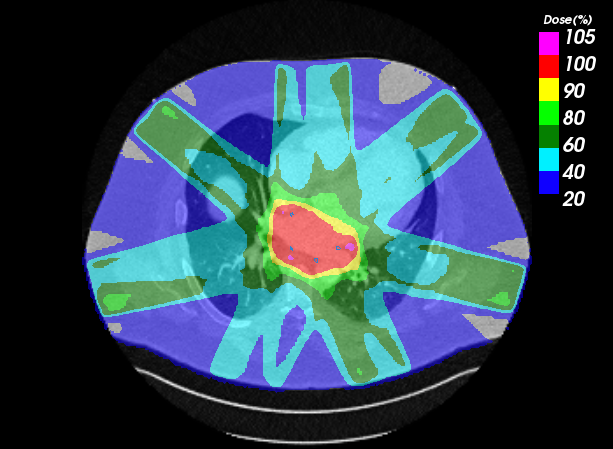
\includegraphics[scale=0.4]{./teile/discussion/Pat05_Amanda.png}
 }
 \subfigure[Patient 2 : carbon ions (IMPT)]{
   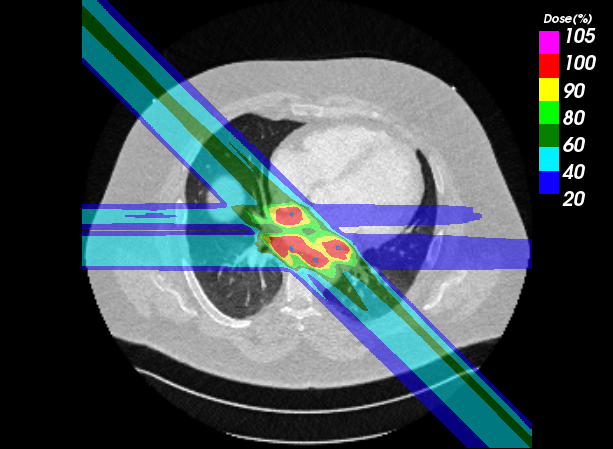
\includegraphics[scale=0.4]{./teile/discussion/Pat05_carbon.png}}
\subfigure[Patient 4 : photons (IMRT)]{
 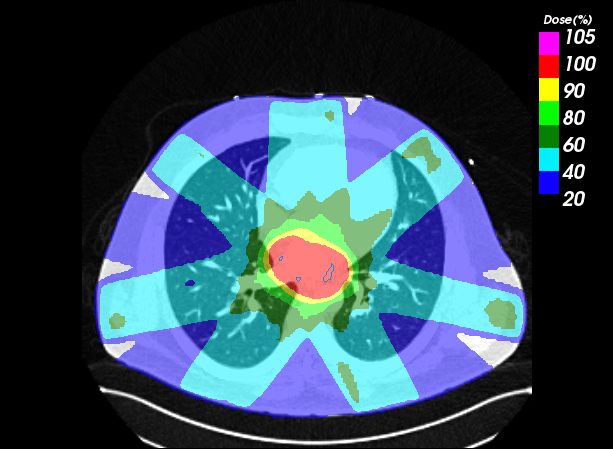
\includegraphics[scale=0.4]{./teile/discussion/Pat08_Amanda.png}}
 \subfigure[Patient 4 : carbon ions (IMPT)]{
  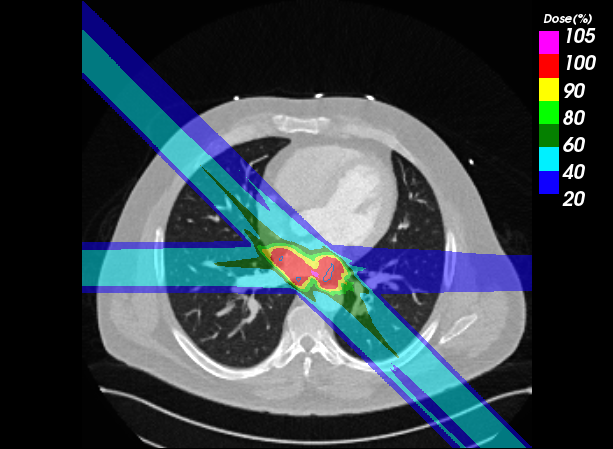
\includegraphics[scale=0.4]{./teile/discussion/Pat08_carbon.png}}
\caption{Comparison of dose cuts with photons (IMRT) and carbon ions (IMPT) treatment are shown for Patient 2 and Patient 4, respectively. 
As target volumes for the LPV and RPV the CTV is displayed. Photon treatment plans are courtesy of Dr. Amanda Deisher, Mayo Clinic, USA. 
The results of both treatment plans are displayed in the software Slicer.} 
\label{dose_IMRT_vs_IMPT}
\end{figure}

% \newpage
\vspace*{-0.3cm}

\begin{table}[H]
\scriptsize
% \tiny
  \centering
  \caption{Dose-volume limits for OARs. The volumes are stated in cc, dose values in Gy. The photon irradiation (IMRT) is compared with two 
  different IMPT setting for carbon ions (weak: maximal 70\% of the physical dose to the esophagus, strong: maximal 30\%). The maximal 
  applicable phyical dose to the target region for the dose-volume limits of the critical structures is stated in the last column for the 
  strong IMPT setting.}
  \begin{tabular}{|c|c||c|c|c||c|c|c||c|}
    \hline\hline
    Patient & OAR & Volume & Dose & endpoint & IMRT & IMPT (weak) & IMPT (strong) & max.D (strong IMPT)\\
    \hline
    2 & Aorta / great vessels & 10 & 31 & Aneurysm & 22.0 & 14.3 & 15.3 & 50.6 \\
    & Esophagus & 5 & 11.9 &  Stenosis / fistula & 24.6 & 22.5 & 7 & 42.5 \\
    & Heart & 15 & 16 & Pericarditis & 27.1 & 25.3 & 30.0 & (13.3) \\
    & Trachea & 4 & 10.5 & Stenosis / fistula & 7.6 & 4.3 & 3 & 87.5 \\
    \hline
    4 & Aorta / great vessels & 10 & 31 & Aneurysm & 21.3 & 8.5 & 6.3 & 123.0 \\
    & Esophagus & 5 & 11.9 &  Stenosis / fistula & 20.2 & 18.5 & 3.5 & 85.0 \\
    & Heart & 15 & 16 & Pericarditis & 26.1 & 24.5 & 22.3 & (18.0) \\
    & Trachea & 4 & 10.5 & Stenosis / fistula & 0 & 0 & 0 & $\infty$\\  
    \hline\hline
  \end{tabular}
  \label{tab:dosevolume:photons:carbon}
\end{table}

\newpage

% \vspace*{1.5cm}

\begin{figure}[H]
\begin{center}
\subfigure[Patient 2 : photons (IMRT)]{
 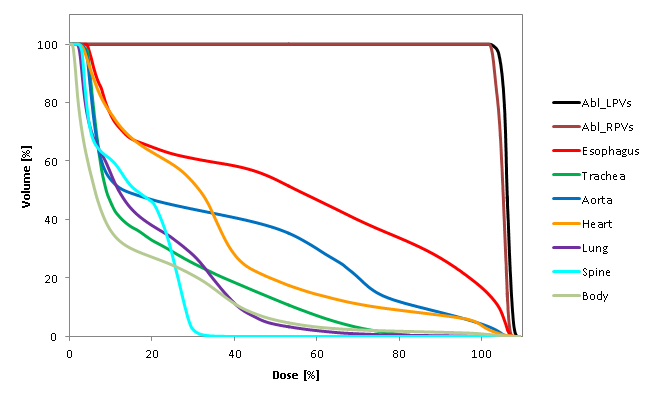
\includegraphics[scale=0.46]{./teile/discussion/Pat05_DVH_Amanda_withLegend.png}
 }
\subfigure[Patient 2 : carbon ions (IMPT)]{
 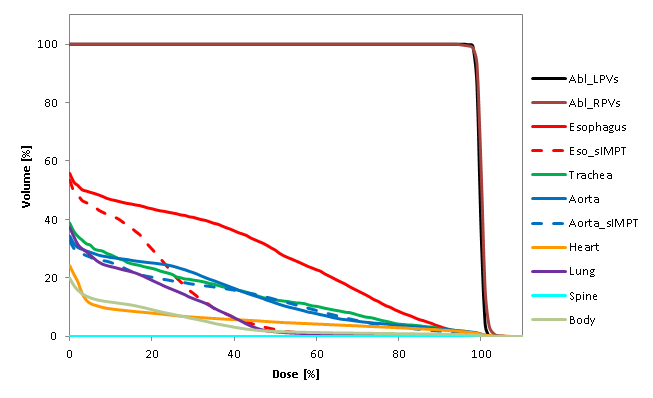
\includegraphics[scale=0.46]{./teile/discussion/Pat05_DVH_carbon_withLegend.png}
 }
\subfigure[Patient 4 : photons (IMRT)]{
 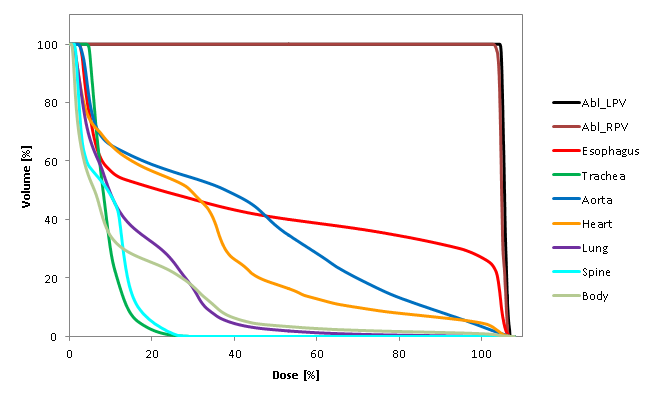
\includegraphics[scale=0.46]{./teile/discussion/Pat08_DVH_Amanda_forLegend.png}
 }
\subfigure[Patient 4 : carbon ions (IMPT)]{
 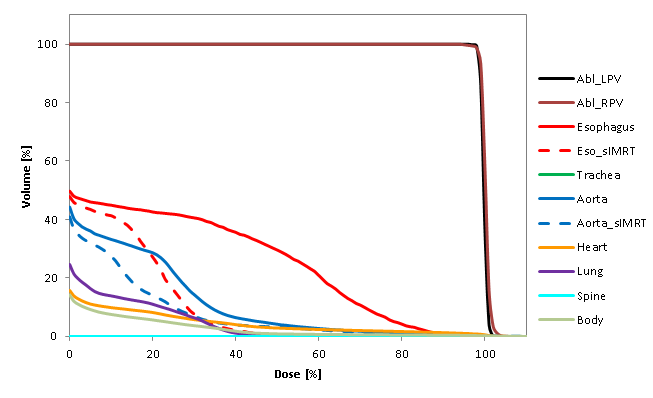
\includegraphics[scale=0.46]{./teile/discussion/Pat08_DVH_carbon_withLegend.png}
 } 
 \end{center}
\caption{Comparison of DVHs are displayed for a treatment with photons (IMRT) versus carbon ions (IMPT). 
Target dose deposition are shown in black for the LPVs and brown for the RPVs, the dose to the esophagus is displayed in red, the trachea dose 
in green, the aorta dose in blue, the heart dose in orange, the lung dose in purple and the spinal cord dose in light blue. Photon treatment 
plans are courtesy of Dr. Amanda Deisher, Mayo Clinic, USA. For the carbon ion treatment plans different IMPT parameters are shown, where 
a better sparing of the esophagus is achieved with stronger limitation parameters, shown in dashed lines.}
\label{dvh_patients_photon_vs_carbon}
\end{figure}

\vspace*{-0.8cm}

\begin{table}[H]
  \centering
  \caption{Integral dose in [Gy$\times$cm$^{3}$] for photon treatment (IMRT) and the two studied IMPT(OAR) deliveries for carbon ion 
  irradiation (weak: maximal 70\% of the physical dose to the esophagus, strong: maximal 30\%).}
  \begin{tabular}{|c|c||c||c|c|}
    \hline\hline
    Patient & OAR & IMRT & IMPT(OAR) (weak) & IMPT(OAR) (strong)\\
    \hline
    2 & Esophagus & 359 & 184 & 80 \\
    & Trachea & 81 & 57 & 48 \\
    & Aorta & 983 & 388 & 356 \\
    & Heart & 13,863 & 2,762 & 2,544 \\
    & Lung & 10,932 & 4,761 & 4,326 \\
    \hline
    5 & Esophagus & 166 & 81 & 32 \\
    & Trachea & 20 & 0 & 0 \\
    & Aorta & 912 & 264 & 180 \\
    & Heart & 6,992 & 1,250 & 1091 \\
    & Lung & 11,274 & 3,126 & 2,730 \\
    \hline\hline
  \end{tabular}
  \label{tab:SID}
\end{table}

\newpage

Due to the different interaction mechanism of photons and ions with matter (see chapter \ref{chapter:intro}, section \ref{intro:imm}), and the 
resulting  inverse depth dose profile of ions the surrounding tissue - including the OARs - can be better spared with carbon ions. Hence 
smaller field channel numbers can be chosen (see figure \ref{dose_IMRT_vs_IMPT}). The sparing of the OAR are shown both in the resulting 
dose-volume deposition to OARs in table \ref{tab:dosevolume:photons:carbon} as well as in the comparison of the resulting DVHs for photons and 
carbon ions (see figure \ref{dvh_patients_photon_vs_carbon}). For the carbon ion study two different IMPT parameter settings were used and 
both results are shown: An IMPT delivery with a weak dose restriction to the esophagus of maximal 70\% of the physical dose of 25Gy and 
an IMPT setting with a stronger restriction of maximal 30\% physical dose to the esophagus. As can be seen in table \ref{tab:dosevolume:photons:carbon} 
the IMPT delivery with the weaker restriction to the esophagus results in dose-volume depositions comparable to the studied photon treatment, while 
the irradiation with the stronger dose restrictions results in a much better sparing of the studied OARs. An exception 
is the heart, as it is also the target volume itself. This structure requires a closer analysis on the irradiated substructures. 
Nevertheless it can already be seen from the DVH information of both patients, that the irradiated heart volume is drastically reduced 
with carbon ions compared to photons, due to the reduced number of beam channels feasible with carbon ions. 
The dose cut images (figure \ref{dose_IMRT_vs_IMPT}) also display that the left ventricles are better 
spared with a non-invasive irradiation of the PVs with carbon ions due to the chosen beam channel directions. It can thus be expected that 
this leads to a better sparing of the radiosensitive left coronary arteries. \newline
\newline
Another method to compare the dose distribution for two different delivery techniques and quality beams is to calculate the integral dose, 
a measure of the total energy absorbed in the treated volume \cite{Kha10}. It is calculated as the product of the mass of the irradiated tissue 
and the absorbed dose. Here, no organ specific density was assumed, but the integral dose was calculated as the dose volume product.  
The results for different critical structures (esophagus, trachea, heart, aorta and lung) are shown in table \ref{tab:SID} 
and it can be seen that the absorbed energy of these organs can be drastically reduced with carbon ions 
compared to photons.

\newpage

\subsubsection{Porcine data}

Photon treatment plans for the irradiation of the AV node were carried out on different CT phases for all four porcine data sets (see chapter 
\ref{chapter:porcine}) as a five field IMRT treatment (see figure \ref{dose_porcine_photon_vs_carbon}) with 6MV photons. In order to keep the 
ITV margin small the center phase of the motion was chosen as planning phase. This resulted in a treatment planning on 70\% of the cardiac 
phase for Pig 1, on 20\% for Pig 2, 0\% (reference phase) for Pig 3 and 70\% for Pig 4. The delivery was also planned as a single fraction 
irradiation of 25Gy. For the ITV additional 3mm isotropic expansions were used, resulting in the final PTV. For a fair comparison the shown 
carbon ion results were calculated on the same CT scan phases. The plans are SFUD irradiations with an isoptropic safety margin of 5mm to the 
CTV. The SFUD carbon ion plans were generated with two opposing beam channel directions (see chapter \ref{chapter:porcine}). The target volume 
as well as the contours of the OAR were kept identical in both deliveries, enabling a direct comparison of the treatment planning outcome.\newline
\newline
The sparing of the OARs are shown both in the resulting dose-volume deposition 
in table \ref{tab:pig:dosevolume:photons:carbon} as well as in the comparison of the resulting DVHs for photons and carbon 
ions (see figure \ref{dvh_porcine_photon_vs_carbon}). Due to the inverse depth-dose profile of carbon ions a reduced number of beam 
channel entry directions is feasible, resulting in a better sparing of the OARs compared to an irradiation of the AV node with photons. 
Due to the used beam channel directions it can be seen that the esophagus as well as the trachea do not receive any dose deposition. 
The dose deposition in the aorta is negligible, resulting in an irradiated volume of less than 10cc. Also the heart itself (which is here 
shown with substracted PTV volume) is much better 
spared with carbon ions, resulting in no dose-volume-limit exceeding irradiation for this structure. For photons on the other hand 
the limit is exceeded in three out of the four studied data sets. It should be noted that the analyzed heart volume excludes the irradiated 
AV node volume and hence also the highest dose deposition, the target dose of 25Gy physical dose.\newline
\newline
Also in the porcine data sets the body was only partially displayed on the CT scans and hence no density information could be derived for the 
calculation of the integral dose. The specific integral dose for both treatment delivery techniques were determined also for these cases. 
Thereby the sum over all dose volume products was calculated for the body contour volume. The results are shown in 
table \ref{tab:SID:pigs} and it can be seen that the absorbed energy to the body volume can be drastically reduced with carbon ions 
compared to photons.

\newpage

\begin{figure}[H]
\centering
\subfigure[Pig 3 : photons (IMRT)]{
 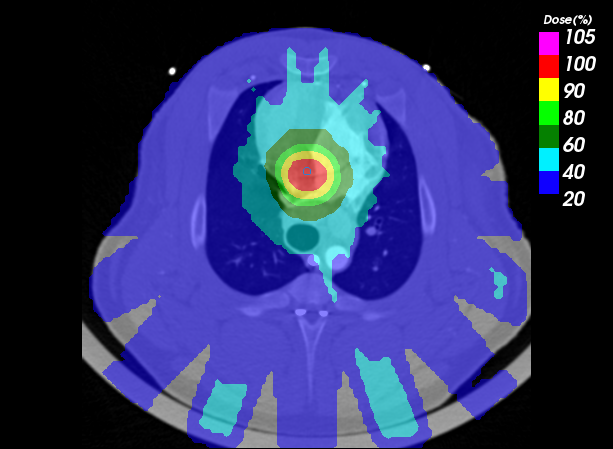
\includegraphics[scale=0.38]{./teile/discussion/L976_IMRT_Limin.png}
 }
 \subfigure[Pig 3 : carbon ions (SFUD)]{
   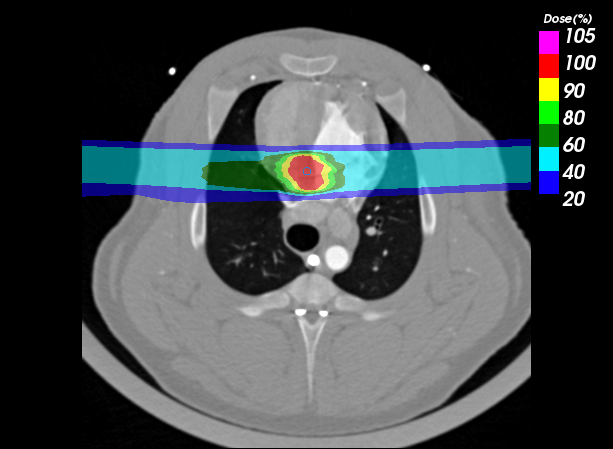
\includegraphics[scale=0.38]{./teile/discussion/L976_carbon.png}
   }
\caption{Comparison of dose cuts with photons and carbon ions treatment are shown for Pig 3. The photon delivery was planned as IMRT treatment 
and the carbon irradiation as SFUD irradiation, respectively. As the AV target volume the CTV is displayed. 
Photon treatment plans are courtesy of Dr.Limin Song, Mayo Clinic, USA. The results of both treatment plans are displayed in the software Slicer.}
\label{dose_porcine_photon_vs_carbon}
\end{figure}

\begin{table}[H]
% \scriptsize
\footnotesize
  \centering
  \caption{
  Dose-volume limits for OARs. The volumes are stated in cc, dose values in Gy. The photon irradiation (IMRT) is compared with SFUD carbon ion 
  irradiation}
  \begin{tabular}{|c|c||c|c|c||c|c|c|}
    \hline\hline
    Pig & OAR & Volume & Dose & endpoint & IMRT & SFUD \\
    \hline
    1 & Aorta / great vessels & 10 & 31 & Aneurysm & 1.1 & 0.0 \\
    & Esophagus & 5 & 11.9 &  Stenosis / fistula & 0.2 & 0.0 \\
    & Heart-PTV & 15 & 16 & Pericarditis & 18 & 6.3 \\
    & Trachea & 4 & 10.5 & Stenosis / fistula & 6.5 & 0.0 \\
    \hline
    2 & Aorta / great vessels & 10 & 31 & Aneurysm & 2.1 & 0.0 \\
    & Esophagus & 5 & 11.9 &  Stenosis / fistula & 0.4 & 0.0 \\
    & Heart-PTV & 15 & 16 & Pericarditis & 16.1 & 6.5 \\
    & Trachea & 4 & 10.5 & Stenosis / fistula & 2.6 & 0.0 \\
    \hline
    3 & Aorta / great vessels & 10 & 31 & Aneurysm & 0.9 & 0.0 \\
    & Esophagus & 5 & 11.9 &  Stenosis / fistula & 0.3 & 0.0 \\
    & Heart-PTV & 15 & 16 & Pericarditis & 23 &  4.8 \\
    & Trachea & 4 & 10.5 & Stenosis / fistula & 0.2 & 0.0 \\
    \hline
    4 & Aorta / great vessels & 10 & 31 & Aneurysm & 0.7 & 0.0 \\
    & Esophagus & 5 & 11.9 &  Stenosis / fistula & 0.3 & 0.0 \\
    & Heart-PTV & 15 & 16 & Pericarditis &  14.3 & 7.3 \\
    & Trachea & 4 & 10.5 & Stenosis / fistula & 4.6 & 0.0 \\
    \hline\hline
  \end{tabular}
  \label{tab:pig:dosevolume:photons:carbon}
\end{table}

\newpage

\vspace*{-0.4cm}
\begin{figure}
\begin{center}
\subfigure[Pig 1]{
 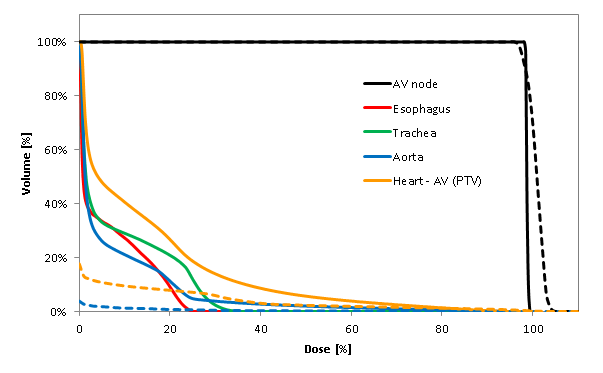
\includegraphics[scale=0.52]{./teile/discussion/L829_DVH.png}
 }
\subfigure[Pig 2]{
 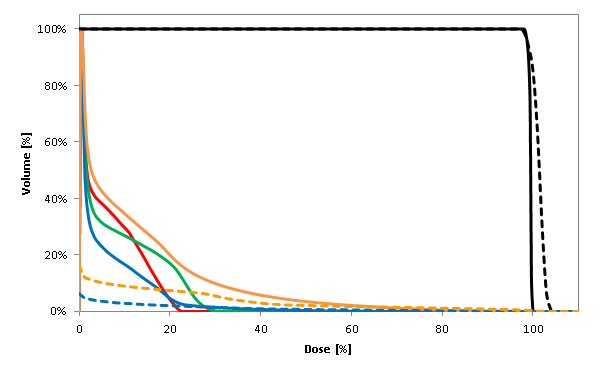
\includegraphics[scale=0.52]{./teile/discussion/L833_DVH_2.png}
 }
\subfigure[Pig 3]{
 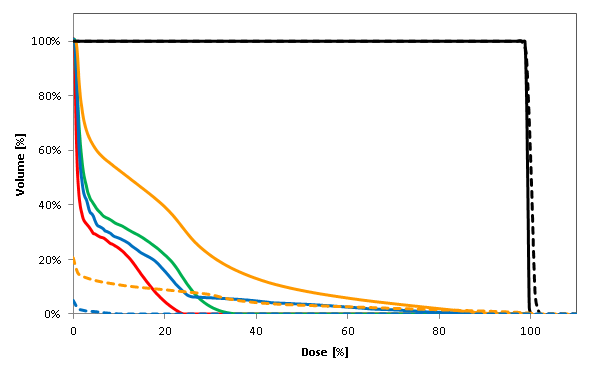
\includegraphics[scale=0.52]{./teile/discussion/L976_DVH_2.png}
 }
\subfigure[Pig 4]{
 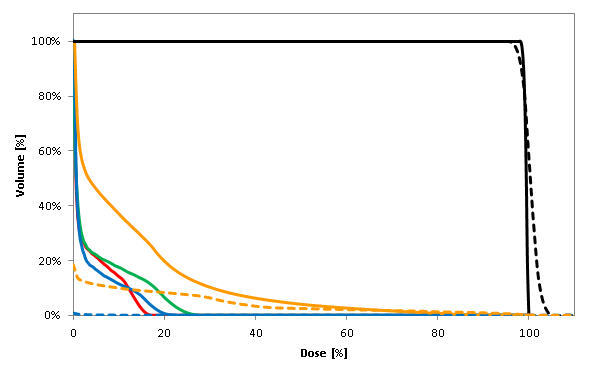
\includegraphics[scale=0.52]{./teile/discussion/L979_DVH_2.png}
 } 
 \end{center}
    \caption{Comparison of DVH results with photons (solid) and carbon ions (dashed). The photon delivery was planned as IMRT treatment 
and the carbon irradiation as SFUD irradiation, respectively. The target dose to the AV node is displayed in black, the dose to the 
esophagus in red, to the trachea in green, the aorta in blue and the irradiated heart (with the substracted PTV volume) is 
shown in orange. In case of carbon SFUD deliveries, the esophagus and trachea do not receive any dose. 
Photon treatment plans are courtesy of Dr. Limin Song, Mayo Clinic, USA.}
\label{dvh_porcine_photon_vs_carbon}
\end{figure}


\begin{table}[H]
% \footnotesize
  \centering
  \caption{Integral dose in [Gy$\times$cm$^{3}$], exemplarily for pig 3, for photon irradiation (IMRT) and carbon ion treatment (SFUD).}
  \begin{tabular}{|c|c||c|c|}
    \hline\hline
    Pig & OAR & IMRT & SFUD  \\
    \hline
    3 & Esophagus & 14 & 0 \\
    & Trachea & 62 & 0 \\
    & Aorta & 66 & 1 \\
    & Heart-PTV & 1,374 & 289 \\
    & Lung & 1,195 & 187 \\
    \hline\hline
  \end{tabular}
  \label{tab:SID:pigs}
\end{table}

\newpage

\section{Treatment planning of cardiac target volumes with scanned ions}

In order to assess the displacement of the cardiac volumes due to respiration and heartbeat, 4DCTs gated on respiration or heartbeat 
were analyzed and the findings will be discussed in section \ref{diss:motion}. Afterwards the usage of contrast enhanced CT scans due to the 
poor contrast between the heart muscle and the contained blood will be discussed in section \ref{diss:ceCT} and possible experimental 
solutions for resulting range uncertainties will be proposed. In section \ref{diss:mmt} the result of the used motion mitigation techniques 
for the irradition of cardiac target volumes with a scanned carbon ion beam will be deliberated. 

\subsection{Motion of cardiac volumes}
\label{diss:motion}

Target volumes in the heart move on one hand due to the respiration of the patient, a motion with a large amplitude and a slow cycle time of 
ten to fifteen respiratory cycles per minute, and on the other hand due to heartbeat, a motion with a small amplitude and cycle time of sixty 
to eighty beats per minutes. Even though both motions occur simultaneously in patients, they were studied independently in the here presented 
treatment planning studies. This can be justified as a CT gated to both motion types would require long CT acquisitions and hence unnecessary 
dose exposures to the patient. 


\subsubsection{PVs motion in humans}

The motion of PVs ablation sites in humans due to respiration were studied based on respiratory gated time resolved computed tomographies 
(4DCTs) of nine lung cancer patients, recorded for radiotherapy at MD Anderson Cancer Center (MDACC), USA. The heartbeat influence was studied 
on cardiac gated 4DCTs of five AF patients, recorded at Mayo Clinic, USA.\newline
\newline
The movement of the ablation sites of the PVs were studied in the three motion directions (superior-inferior (SI), anterior-posterior (AP) 
and left-right (LR)) as well as for the absolute displacement. Different studies concerning the PVs displacement due to respiration can also 
be found in literature \cite{Ect08, Nos05}, as breathing is also relevant for cather ablation due to the reduction in catheter 
tip contact force \cite{Kum12}. While Ector et al. stated an absolute mean displacement of (19.1 $\pm$ 8.6)mm for both LPV and RPV, 
a much smaller absolute mean displacement of (6.8 $\pm$ 3.6)mm and (6.8 $\pm$ 2.5) was found in the here studied patient cohort for LPV 
and RPV, respectively. The SI motion was the biggest motion direction with a mean displacement of (-6.4 $\pm$ 3.8)mm for LPV 
and (-6.6 $\pm$ 2.4)mm for RPV. AP and LR directions were almost negligible with a mean motion of less than 2mm. 
The difference between the two cardiac sites is more pronounced in AP and LR, so that, e.g., the LPV move more in 
anterior direction. In LR direction a difference between LPV and RPV motion resulted, where the mean displacement of the LPV is 
almost double compared to the RPV. Ector et al. on the other hand found a mean displacement of (14.6 $\pm$ 7.7)mm in inferior direction, 
(9.7 $\pm$ 7.6)mm in anterior direction and (0.4 $\pm$ 3.8)mm in the left direction, hence concluding a much bigger displacement in SI and AP 
directions. It remains to be analyzed if this discrepancy is due to the here studied lung tumor patient cohort in comparison to the AF 
patients studied by Ector et al.. Nevertheless it should be noted that both analyses are based on a small patient number (nine patients 
and sixteen patients, respectively).\newline
\newline
The motion of the ablation sites for the PVs due to heartbeat was studied for the left and right structures, respectively, in the three 
above stated motion directions. Only a small mean absolute displacement over all patients of less than 3mm was observed. The biggest 
absolute displacment reached a mean value of up to (6.5 $\pm$ 3.0)mm in one patient case for the RPV and (5.5 $\pm$ 3.1)mm for the LPV. 
No dominant motion direction was found, even though a tendency to a bigger motion in AP direction could be assumed. Furthermore, no motion 
pattern could be derived from the five studied patient data sets, indicating that the underlying motion causing the PV ablation sites to 
move is much more complex and the result of different motion influences. For further studies concerning the PV displacement due to 
heartbeat, the reader should be refered to Lickfett et al. \cite{Lic05} and Patel et al. \cite{Pat08}. 
Lickfett et al. found comparable maximal displacements of up to 7.2mm in some of the healthy volunteers. Patel et al., who studied 
the displacement in thirty AF patients, stated mean values in the order of 3mm. The here presented results are hence in good agreement 
with the literature values. 

\subsubsection{Motion in porcine due to heartbeat}

The motion of different potential cardiac ablation sites (AV node, CTI and PVs) were studied in pigs based on cardiac gated 4DCTs of four 
swines, recorded at Mayo Clinic, USA. The acquired CT scans were both native and contrast enhanced. It was found that native CT scans 
do not enable an assessment of the cardiac target volume displacement due the low contrast between the cardiac muscle and the contained blood. 
Analysis was hence carried out on the contrast enhanced CT scans. Concerning the motion of the three studied potential target sites 
it could be stated that the PVs moved to the smallest extent (maximal displacement of up to 5mm), followed by the AV node (maximal 
displacement of up to 6mm) and that the CTI moved the most (maximal displacement of 7mm). It was speculated that 
this is due to the location of the volumes, where a proximal location on or near the ventricles lead to a larger movement. 
Even though also in the porcine data sets no maximal motion phase or motion pattern could be observed due to heartbeat it was found that the displacement was 
shallower between certain motion phases (motion phase 6 to 13) and hence, contrary to the studied human data, gating could be an optional 
motion mitigation technique. Moreover, in comparison to the human data, the displacement in AP direction in the porcine data was clearly 
larger than in the other two studied directions. 


\subsection{Contrast enhanced CT scans}
\label{diss:ceCT}

Particle treatment planning needs to be carried out on native CT scans in order to obtain the correct range information \cite{Wer04}. In case 
of the intended irradiation of cardiac target volumes it was found that native CT scans do not provide sufficient contrast between the  
heart muscle and the contained blood. As stated, the motion information can thus only be assessed from contrast-enhanced CT scans. 
It needs to be studied if the displacement vector field obtained from registration on the contrast enhanced CT scans yield a good enough 
agreement when directly used on the native data sets for the actual treatment planning. 
The resulting range uncertainties need to be carefully considered, especially regarding the dose to critical structures like the esophagus. 
Analog to studies by e.g. el Bentefour et al. \cite{Bent12}, where in vivo range verifications were 
successfully achieved with a small dose deposition (<0.5cGy) in silicone diodes, a possible solution could be to predeposit the resulting 
treatment plan with a small dose in the order of mGy. By placing such an detector with a catheter inside the patient, either in front of 
or inside the esophagus, it would allow to test for range of the planned energies and hence for potential miscalculation or 
interfractional changes of the organs. Range uncertainties to the target area could furthermore be corrected before irradiation with the 
total single fraction dose. By using in-beam PET monitoring with $^{11}$C and $^{10}$C fragments (see chapter \ref{chapter:intro}, section 
\ref{intro:nt}) it would be possible to irradiate a low dose in order to detect the range and position uncertainties. This was already carried 
out at GSI, where $^{10}$C resulted to be best suited as a probing beam for range verifications \cite{Lin12}. 
The accuracy of PET monitoring for ion range determination was studied by Fiedler et al. \cite{Fie10} for more than 80 of the 400 patients 
irradiated in the GSI pilot project. It was stated that in-beam PET method demonstrated a high sensitivity for the 
detection of range deviations and would thus be beneficial for the here presented treatment modality. 


\subsection{Motion mitigation techniques}
\label{diss:mmt}

Due to the large motion of the PV ablation sites induced by the respiratory motion in the studied patient cohort, interplay was observed to 
lead to strong underdosage, so that in some cases only V95=70\% was achieved with no safety margin and V95=80\% with safety margins of 
5mm. Due to the large motion amplitude of more than 1cm gating was studied as potential motion mitigation technique (see next paragraph). 
For the displacements induced by heartbeat a smaller motion of less than 1cm was observed in all studied human data, so that rescanning was studied 
as an adequate motion mitigation technique for this case. As expected, the interplay effect in this case was smaller than for respiration, 
with minimal underdosages of V95=85\% for no safety margin and a minimal V95 of 92\% for 5mm and 7mm margin, respectively. 
Even though this underdosage with safety margin already yields a clinically acceptable dose coverage the usage of an additional motion 
mitigation technique leads to a more robust treatment delivery. For the porcine data, where the motion influence of the heartbeat on the AV 
node target volume 
was studied and only a single margin of 5mm was used, the interplay effect led to larger minimal underdosages of 56\% in some of the studied 
pig data sets. Hence the usage of rescanning as motion mitigation technique was needed in this case as well. 


\subsubsection{Respiratory motion}
\label{diss:resp:mmt}

In the animal model studies by Sharma et al. \cite{Sha10} the target displacement due to respiration was tracked with the CyberKnife 
system. In the study by Blanck et al. \cite{Bla13} an ITV approach was used for the respiratory motion. Here, gating was used as a potential 
motion mitigation technique. It is suited for larger target displacments, since only a fraction of the motion cycle is used. The gating window 
is positioned at end exhale, enabling a more robust delivery with only a small amount of residual motion. 
To this date, gating is already used in ion beam centers with passive particle delivery \cite{Min00} as well as in IMRT treatments 
in photon centers \cite{Kea06}. A pilot study with scanned carbon ions was recently conducted on liver patients at HIT by using gating and 
abdominal compression \cite{Ric12}. In the here studied case, gating was found to be an adequate motion mitigation technique so that underdosages could be increased up to 
a minimum of 98\% for all studied safety margins and patient cases. Even in cases with no safety margin underdosage could be increased to a 
minimum of 94\%. It can nevertheless be stated that safety margins, which are needed in order to account for e.g. position inaccuracies, 
improved the outcome and made the delivery more robust. It was furthermore studied in two patient data sets if the treatment outcome improved 
when rescanning was applied for the residual motion inside the gating window. This is proposed as phase-controlled rescanning \cite{Fur07} or 
breath-sampled rescanning \cite{Sec09}. It resulted in a marginal improvement compared to only gating, whereas no improvement was observed when 
using more than ten rescans. Since the irradiation of the PV ablation sites were also studied to include rescanning as mitigation for heartbeat motion, the 
combination of these two techniques will be automatically achieved. Concerning the treatment time it was expected that gating would increase the 
treatment time dependence on the used gating window. Since only 30\% of the motion cycle was used for irradiation, the treatment 
resulted into a delivery time of about 30min with a high intensity of 55,000 minimum particles per beam spot and for a safety margin of 3mm. 
Compared to the radiofrequency ablation procedure which takes up to a couple of hours, and to the photon irradiation of up to two hours 
\cite{Sha10}, the treatment time is drastically reduced. This was found for the HIT beam parameters, where a relatively long time for an 
energy change is needed. The particle intensity could be further increased, leading to an even further reduced treatment time. Nevertheless 
it was shown that very high intensities can endanger a homogenous dose coverage \cite{Mue14}. New accelerator concepts with variable 
excitation cycles \cite{Tsu08} or faster energy changes \cite{Iwa10} might hence be needed. 
An alternative to gating could be the usage of apneic oxygenation, which is currently used at the Rinecker Proton Therapy Center in Munich 
\cite{Ber11, RPTC12} for the treatment of tumors in the upper abdomen and thorax. This approach will also be used in the planned animal experiments 
with pigs which will be carried out at GSI in the summer of 2014. 

\subsubsection{Heartbeat motion}
\label{diss:hb:mmt}

In the animal model studies by Sharma et al. \cite{Sha10} and by Blanck et al. \cite{Bla13} an ITV approach was used for the heartbeat motion. 
In the here presented study rescanning was used as a motion mitigation technique for heartbeat motion, both in human as well as for 
the porcine data sets. Especially in human data only rescanning seemed to be an adequate technique due to the lack of a motion pattern 
or a region of shallower motion. For the porcine data on the contrary, cardiac gating might be another option, which needs to be investigated. 
In the human data it was found that the dose coverage was higher than 99\% in about 96\% of the studied cases with safety margins over 3mm. 
This result could be even further improved if ten or more rescans were applied. Nevertheless it can be argued that five rescans already 
yield a very good dose deposition in the target volume. For the porcine data and the studied AV node ablation it was found 
that the dose coverage was higher than 99\% in 85\% of the studied cases with a safety margin of 5mm. This finding could be slightly improved to 
91\% of the studied cases for ten rescans. A higher rescan number of fifteen rescans did not lead to a significant improvement. 
The finding indicates that ten rescans are already sufficient to enable a robust and 
stable irradiation of the cardiac target volume in the presence of heartbeat. Due to the high single dose the resulting intensity per rescan 
is expected to be large and hence the application should be feasible without further prolonging the treatment time. 
All the studied rescanning results were obtained for slice-by-slice rescanning. This means that each IES is rescanned independently with the 
predefined numbers of rescans. In other studies it has nevertheless be found that other rescan methods, like e.g. breath-sampled rescanning 
\cite{Sec09} or phase-controlled rescanning \cite{Fur07}, result in an increased robustness while requiring fewer rescan numbers compared to 
slice-by-slice rescanning as it breaks up possible synchronicities between beam application and target motion \cite{Mue14}. In breath-sampled 
rescanning the IES are rescanned individually, but the rescans are sampled according the motion phase of the breathing period, so that every 
motion phase receives dose appliactions. An analog delivery according to the heartbeat and hence an ECG-sampled rescanning might be feasible 
and could lead to improved results. 

